\chapter{Implementación}\label{ch:implmentacion}
%************************************************
Una vez habiendo establecido tanto la estructura como distintos conceptos de implementación, se puede empezar a incidir sobre diferentes implementaciones realizadas. El código fuente del proyecto, como he explicado en el capítulo anterior, está alojado en la plataforma de GitHub bajo el enlace de \url{https://github.com/nikitastetskiy/Wrapped}, el \textit{Back-end} en la plataforma Heroku bajo el enlace de \url{https://wrappedtrends.herokuapp.com} y el \textit{Front-end} en la plataforma Vercel bajo el enlace de \url{https://wrapped-trends.vercel.app}. Aún así, es conveniente analizar y explicar los diferentes códigos fuentes y algoritmos que se han implementado a lo largo del proyecto.

\section{Implementación Back-end}
La implementación de las capas pertenecientes a \textit{Back-end} se localizan en los directorios \textit{app} y \textit{backend}. El primero, guarda todas las entidades y \textit{scripts} necesarios para la obtención y gestión de datos de las tendencias. Mientras que el segundo guarda toda la estructura del servicio del servidor y el modelo perteneciente a la base de datos.

\subsection{Implementación Principal}
La primera implementación de código que se estudiará será la función principal encargada de gestionar las tendencias. Está denominada bajo el nombre de \textit{main\_operation}. Dicha función consigue las tendencias acordes al país y construye el diccionario apropiado, dependiendo de si existe dicho país en la base de datos o no. Si existe se tendrá que hacer una llamada de edición o PUT, en cambio si no existe se tendrá que crear y hacer una llamada POST. Además, se comprueba si existe un país con una antigüedad de más de 7 días para eliminarlo, con el objetivo de optimizar la base de datos.

\vspace{0.3cm}

En este primer caso, creo que es conveniente mostrar tanto el pseudocódigo como el código fuente de la función. En casos posteriores se alternará en base a la relevancia de la función, con el fin de optimizar la comprensión lectora.

\begin{algorithm}[H]\label{alg:offspring_fs}

    \Fn{Main}{

        \KwIn{country}
        trends $\longleftarrow$ getTrends(country)\;
        \If{\textit{trends}}{
            today = datetime.now(country)\;
            yesterday = today - 1\;
            oldCountry = requests.get(\textit{URI\_ENDPOINT})\;
            \If{oldCountry}{
                dict $\longleftarrow$ createDictCountry(country, trends, today, yesterday, oldCountry)\;
            } \Else{
                dict $\longleftarrow$ createDictCountry(country, trends, today, yesterday)\;
            }
            \If{\textit{dict}}{
                \If{oldCountry}{
                    requests.put(\textit{URI\_ENDPOINT}, dict.json())\;
                } \Else{
                    requests.post(\textit{URI\_ENDPOINT}, dict.json())\;
                    sevenDaysOldCountry = requests.get(\textit{URI\_ENDPOINT})\;
                    \If{\textit{sevenDaysOldCountry}}{
                        requests.delete(\textit{URI\_ENDPOINT})\;
                    }
                }
            }
        }
    }

    \caption{Operación Principal}

\end{algorithm}
\vspace{0.3cm}

La función tiene por \textit{input} \textit{country}, el cual es un diccionario con valores predefinidos que necesita cada país, es decir, valores como el nombre del país, el WOEID, el código del país, su lenguaje y su zona horaria. Otro valor predefinido es el \textit{endpoint} de mi servidor, para realizar llamadas HTTP.

\vspace{0.3cm}

\begin{lstlisting}[caption=Operación principal,          label={lst:listing-python},language=Python]
def main_operation(country):

    sorted_trends = get_trends_with_country(country['woeid'])
    if sorted_trends:

        DATE = datetime.now(
            timezone(country['timezone'])).strftime("%y-%m-%d")
        YESTERDAY = (datetime.now(timezone(country['timezone']))
                    - timedelta(days=2)).strftime("%Y-%m-%d")
        resp = requests.get(f"{TRENDING_WRAPPED_ENDPOINT}
                {country['name']}/{DATE}")

        # Checking if the object exists already
        if resp.status_code == 200:
            my_dict = create_dict_country(country,
                        sorted_trends, DATE, YESTERDAY,
                        json.loads(resp.content)["tendencias"])

        else:
            my_dict = create_dict_country(
                country, sorted_trends, DATE, YESTERDAY, False)

        if my_dict:
            my_dict_json = json.dumps(
                my_dict, default=lambda o: o.__dict__)
            my_headers = {
                'accept': 'application/json',
                'Content-Type': 'application/json'
            }
            # Checking if the object exists already
            if resp.status_code == 200:
                req = requests.put(
                    TRENDING_WRAPPED_ENDPOINT, data=my_dict_json,
                    headers=my_headers)
            else:
                req = requests.post(
                    TRENDING_WRAPPED_ENDPOINT, data=my_dict_json,
                    headers=my_headers)
                OLD_DATE = (datetime.now(timezone(
                            country['timezone'])) -
                            timedelta(days=7)).
                            strftime("%y-%m-%d")
                old_resp = requests.get(
                    f"{TRENDING_WRAPPED_ENDPOINT}
                    {country['name']}/{OLD_DATE}")
                # Checking for old objects
                if old_resp.status_code == 200:
                    old_resp = requests.delete(
                        f"{TRENDING_WRAPPED_ENDPOINT}
                        {country['name']}/{OLD_DATE}")
\end{lstlisting}

Para la creación de los diccionarios, el \textit{endpoint} y el acceso a la API de Twitter se han creado unas constantes globales. Se ha propuesto tres países relevantes como ejemplos. En cuanto al acceso a la API de Twitter se puede hacer de varias maneras, pero las funciones y los recursos de la API cambian dependiendo de la manera que se autentifique en la API. En este caso se ha hecho con V1, pero también se ha comentado la otra posibilidad.

\vspace{0.3cm}

\begin{lstlisting}[caption=Declaraciones de paises,          label={lst:listing-python},language=Python]
COUNTRIES = [
    {
        'name': 'Spain',
        'woeid': 23424950,
        'code': 'ES',
        'language': 'es',
        'timezone': 'Europe/Madrid'
    },
    {
        'name': 'United States',
        'woeid': 23424977,
        'code': 'US',
        'language': 'en',
        'timezone': 'US/Pacific'
    },
    {
        'name': 'Ukraine',
        'woeid': 23424976,
        'code': 'UA',
        'language': 'uk',
        'timezone': 'Europe/Kiev'
    }
]
\end{lstlisting}

\begin{lstlisting}[caption=Declaración de \textit{endpoint},          label={lst:listing-python},language=Python]
TRENDING_WRAPPED_ENDPOINT = "https://wrappedtrends.herokuapp.com/country/"
\end{lstlisting}

Cada proyecto iniciado en la API de Twitter proporciona claves de acceso o secretos únicos que no deben ser compartidos con nadie. Estos son utilizados para acceder y autenticarse en la API.

\vspace{0.3cm}

\begin{lstlisting}[caption=Autentificación de la API de Twitter,          label={lst:listing-python},language=Python]
# ENV VARIABLES OF TWITTER API
consumer_key = os.getenv('API_KEY')
consumer_secret = os.getenv('API_SECRET')
access_token = os.getenv('ACCESS_TOKEN')
access_token_secret = os.getenv('ACCESS_TOKEN_SECRET')

# TWITTER API
auth = tweepy.OAuthHandler(consumer_key, consumer_secret)
auth.set_access_token(access_token, access_token_secret)
api = tweepy.API(auth)

# client = tweepy.Client(bearer_token=BEARER_TOKEN)
\end{lstlisting}

La operación principal se tendrá que ejecutar para cada país, lo cual es bastante costoso, debido a que cada país o valor del diccionario tendrá que estar esperando hasta la finalización del valor que haya por delante. Debido a esto he implementado una función que se ejecute mediante el multiprocesamiento. La función recorre los diferentes países de manera asíncrona, bajo la premisa del número máximo de procesos que se pueden utilizar para ejecutar las llamadas dadas, en el caso dado es 200. Si no se proporciona, se crearán tantos procesos de trabajo como procesadores tenga la máquina.

\vspace{0.3cm}

\begin{lstlisting}[caption=Ejecución con multiprocesamiento,          label={lst:listing-python},language=Python]
def main():

    # Multiprocessing
    executor = concurrent.futures.ProcessPoolExecutor(200)
    futures = [executor.submit(main_operation, country) for country in COUNTRIES]
    concurrent.futures.wait(futures)

if __name__ == "__main__":

    main()
\end{lstlisting}


Por lo que algo que puede tardar minutos en ejecutarse de manera síncrona, lo hace en menos de un tercio de tiempo debido al multiprocesamiento, aunque la consumición de energía del procesador es mayor. En la siguiente imagen se pueden ver los resultados, la primera imagen será sin el multiprocesamiento y la segunda lo incluirá.

\begin{figure}[H]
    \centering
    \myfloatalign
    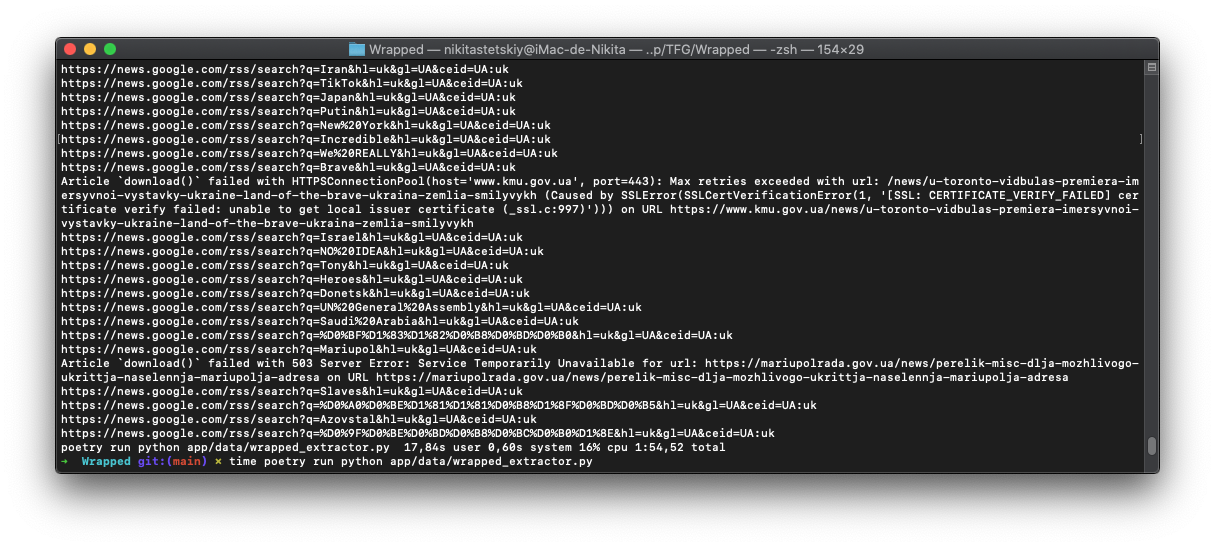
\includegraphics[width=1\textwidth]{gfx/comparacion-multiprocesamiento.png}
    \caption[Comparación de la ejecución sin multiprocesamiento]{Comparación de la ejecución sin multiprocesamiento.}\label{gfx:comparacion-multiprocesamiento}
\end{figure}

Aunque el mayor coste de la ejecución se basa en la descarga de diferentes artículos o noticias en base a la tendencia, esto es debido a que dependen del ancho de la red y su velocidad de descarga, la implementación de la función correspondiente se verá más adelante.

\begin{figure}[H]
    \centering
    \myfloatalign
    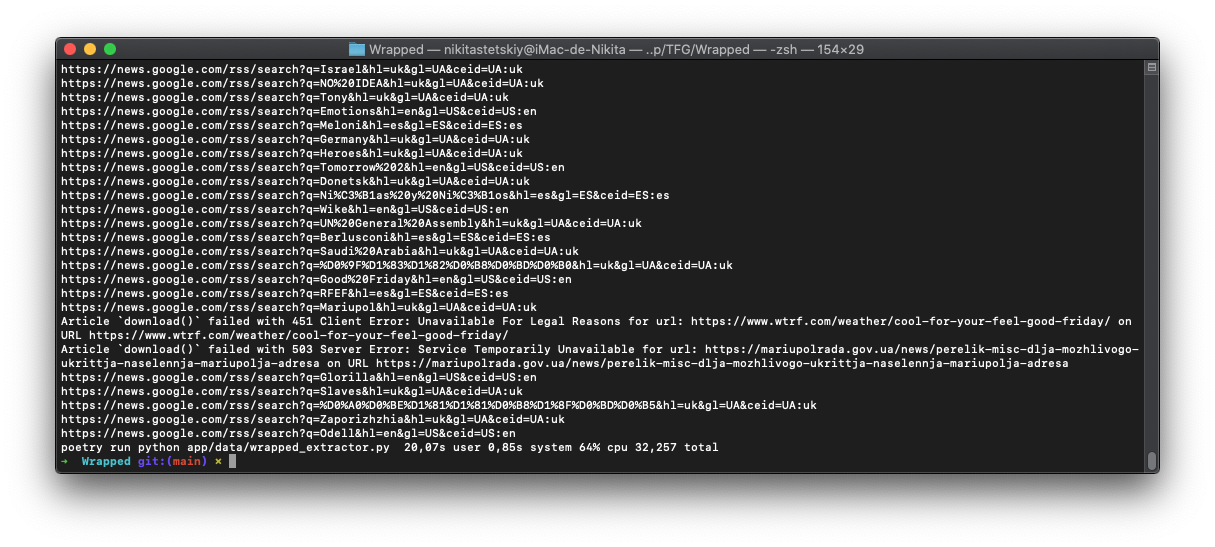
\includegraphics[width=1\textwidth]{gfx/comparacion-multiprocesamiento2.png}
    \caption[Comparación de la ejecución con multiprocesamiento]{Comparación de la ejecución con multiprocesamiento.}\label{gfx:comparacion-multiprocesamiento2}
\end{figure}

\subsection{Implementación de la Generación del Diccionario}
La generación del diccionario a simple vista puede parecer sencilla, ya que solo tenemos que descargar los nombres de las tendencias y convertirlos en distintos objetos para que la base de datos pueda interpretarlos. Aunque esto se puede complicar debido a varios factores.

\vspace{0.3cm}

Primero, si se tiene un objeto ya creado en la base de datos, pues se tendrá que descargarlo y compararlo con el nuevo. Esto es debido a que las tendencias cambian cada hora y se debe tener en cuenta las tendencias viejas y sus distintos atributos. Por lo que se hará una unión entre las tendencias nuevas y las viejas, y posteriormente una diferencia simétrica entre las tendencias restantes con el objetivo de actualizar los atributos de tendencias viejas o incorporar tendencias completamente nuevas. Luego, se tiene que realizar distintas llamadas con distintos parámetros a la API de Twitter, con la intención de crear diferentes objetos funcionales y agregarlos al diccionario (objetos como la popularidad, los sentimientos o artículos).

\vspace{0.3cm}

Al descargar tendencias nuevas y compararlas con las viejas, se hará unión si hay tendencias bajo el mismo nombre. Esto es debido a que es necesario actualizar atributos como la popularidad, pero a la vez mantener el historial del volumen de publicaciones. Luego, la diferencia simétrica se refiere a las tendencias que no aparecen en la unión, ellas también estarán en cuenta a la hora de ordenar la lista de tendencias bajo el valor de la popularidad.

\begin{algorithm}[H]

    \Fn{createDictCountry}{

        \KwIn{country, sortedTrends, date, yesterday, oldTrends}
        \KwOut{dictCountry}
        sortedParsed $\longleftarrow$ $\emptyset$\;
        hour = datetime.now(country)\;
        cont = 0\;
        \If{\textit{oldTrends}}{
            sortedParsed $\longleftarrow$ parseTrend(sortedTrends) $\cup$ oldTrends\;
            sortedParsed $\longleftarrow$ sortedParsed $\triangle$ oldTrends\;
        } \Else{
            sortedParsed = parseTrend(sortedTrends)
        }
        \While{cont $\neq$ 10}{
            tweets $\longleftarrow$ api.searchTweets($sortedParsed_{cont}$)\;
            keywords $\longleftarrow$ searchKeywords(tweets)\;
            sentiments $\longleftarrow$ searchSentiments(tweets)\;
            articles $\longleftarrow$ searchArticles(tweets)\;
            cont++\;
        }
        dictCountry = dictCountry(keywords, sentiments, articles)\;
        \KwRet dictCountry\;
    }

    \caption{Creación del Diccionario Country}

\end{algorithm}

\vspace{0.3cm}

Habiendo entendido el pseudocódigo podemos comprender de una manera más sencilla el código fuente. Primero se comprueba si existen tendencias viejas, después se procedería a asignar una estructura constituyente a dichas tendencias mediante la unión y la diferencia simétrica. Además, sólo se procede al final con 20 tendencias y se calcula su popularidad, esto es debido a la optimización de la base de datos y su gestión. Posteriormente se calculan los demás valores (keywords, sentimientos y artículos) sobre la mitad de las tendencias clasificadas, es decir, un top 10. Las otras diez tendencias, que no llegaron a clasificarse, sirven como referencia posteriormente a la hora de pintar el gráfico de la popularidad, ya que esa información sigue siendo relevante, como historial, si la tendencia llega a ser mostrada.

\vspace{0.3cm}

\begin{lstlisting}[caption=Creación de la estructura de tendencias,          label={lst:listing-python},language=Python]
if old_trends:
    for item in sorted_trends:
        t = parse_trend(item['name'], item['tweet_volume'],
        hour, None)
        for k, old_item in enumerate(old_trends):
            if old_item["name"] == item["name"]:
                t.popularity.refresh(old_item["popularity"]
                        ["volume"],old_item["popularity"]
                        ["hour_popularity"])
                old_trends.pop(k)
                break
        sorted_parsed.append(t)
    for i in old_trends:
        sorted_parsed.append(Trend(**i))

# When there aren't any new trends on the platfrom yet
else:
    for item in sorted_trends:
        t = parse_trend(item['name'], item['tweet_volume'],
            hour, None)
        sorted_parsed.append(t)

sorted_parsed = comparing_names(sorted_parsed)
sorted_parsed = sorted(sorted_parsed, key=lambda trend:
    trend.popularity.peak_popularity, reverse=True)[:20]
\end{lstlisting}

Una vez teniendo la estructura y los objetos de las tendencias, podemos proceder a calcular los demás valores, donde necesitaremos descargar como máximo cien publicaciones o tweets relacionadas con la tendencia. Primero se hace una llamada a la API con determinado valor hacia el ámbito popular. Se filtran las publicaciones repetidas y se intenta que sean publicaciones populares, si no se consiguen se opta por publicaciones menos famosas. Además, sólo se procede a asignar los valores una vez habiendo calculado todos ellos, para que solo existan objetos completos a la hora de visualizarlos.

\vspace{0.3cm}

\begin{lstlisting}[caption=Creación de la estructura constituyente,          label={lst:listing-python},language=Python]
wts = 0
while wts < 10 and cont < len(sorted_parsed):
    name = sorted_parsed[cont].name
    tweets = api.search_tweets(q=f'{name} -filter:retweets
            min_faves:20 since:{yesterday}', lang=country
            ["language"], count=100, result_type="mixed",
            tweet_mode="extended")
    if (len(tweets)) < 50:
        tweets = api.search_tweets(q=f'{name} -filter:retweets
            since:{yesterday}', lang=country["language"],
            count=100, result_type="mixed",
            tweet_mode="extended")
    t = get_tweets(tweets, country["language"])
    if t:
        name = more_specific_name(t.words, name)
        w = get_wrappeds(name, country["code"],
            country["language"])
        if w:
            s = get_sentiments(tweets, country["language"],
                t.label)
            if s:
                sorted_parsed[cont].wrappeds = w
                sorted_parsed[cont].keywords = t
                sorted_parsed[cont].sentiments = s
                wts += 1
    cont += 1

dict_country = {
    'pais': country["name"],
    'dia': date,
    'tendencias': sorted_parsed
}

return dict_country
\end{lstlisting}

La búsqueda de un tópico funcionaría de la misma manera, pero solo consiguiendo un solo objeto completo. También se limita el cálculo de la popularidad, ya que esa información proviene de las tendencias de la API de Twitter. Por lo que las únicas diferencias a la hora de implementarlo serían las funciones de estructuración.

\vspace{0.3cm}

\begin{lstlisting}[caption=Estructuración de la tendencia,          label={lst:listing-python},language=Python]
# PARSING OBJECT TREND
def parse_trend(name, vol, time, array):

    popularity = parse_popularity(vol, time)

    values = {
        'name': name,
        'popularity': popularity,
        'wrappeds': array
    }

    return Trend(**values)

# PARSING OBJECT SINGLE TREND
def parse_single_trend(name, array):

    values = {
        'name': name,
        'popularity': None,
        'wrappeds': array
    }

    return Trend(**values)
\end{lstlisting}

A la hora de descargar las tendencias de Twitter, se tiene que comparar los nombres de distintas tendencias tal como se ha comentado en las tareas de la Historia de Usuario del Sprint 2 (\ref{subs:sprint-2}). Para ello se comprueban si hay parecidos en los nombres, sin contemplar las mayúsculas, minúsculas y tildes. Por lo que para ello se han creado dos funciones, una normaliza una oración (quitando tildes, mayúsculas y caracteres de puntuación) y la otra recorre las distintas tendencias en busca de parecidos.

\vspace{0.3cm}

\begin{lstlisting}[caption=Comprobación de los nombres de tendencia,          label={lst:listing-python},language=Python]
def normalize_str(c):
    s = string.punctuation + " "
    return c.translate(str.maketrans("áéíóú","aeiou", s)).lower()

def comparing_names(s):
    i = 0
    while i < (len(s)-1):
        j = i+1
        while j < (len(s)):
            if normalize_str(s[j].name) in normalize_str(s[i].
            name) or normalize_str(s[i].name) in 
            normalize_str(s[j].name):
                if len((s[i].name).split()) > len((s[j].name).
                split()):
                    s.pop(j)
                    j -= 1
                elif len((s[i].name).split()) < 
                len((s[j].name).split()):
                    s.pop(i)
                    i -= 1
                    break
                else:
                    if s[j].popularity.peak_popularity >= s[i].
                    popularity.peak_popularity:
                        s.pop(i)
                        i -= 1
                        break
                    else:
                        s.pop(j)
                        j -= 1
            j += 1
        i += 1

    return s
\end{lstlisting}

\subsection{Implementación de la Popularidad}
La entidad Popularidad está compuesta por distintos valores comentados en la sección \ref{subsub:ent-popularidad}. Dentro de la entidad Popularidad está la función que actualiza los valores y se calculan con una librería popular orientada hacia campo matemático llamada \textit{numpy}.

\vspace{0.3cm}

\begin{lstlisting}[caption=Estructuración de la popularidad,          label={lst:listing-python},language=Python]
# PARSING OBJECT POPULARITY
def parse_popularity(vol, time):

    values = {
        'volume': [vol],
        'hour_popularity': [time],
        'avarage_popularity': vol,
        'peak_popularity': vol,
    }

    return Popularity(**values)
\end{lstlisting}

\begin{lstlisting}[caption=Actualización de la popularidad,          label={lst:listing-python},language=Python]
def refresh(self, vol, hour):
    self.volume = vol + self.volume
    self.hour_popularity = hour + self.hour_popularity
    self.avarage_popularity = int(np.average(self.volume))
    self.peak_popularity = int(np.max(self.volume))
\end{lstlisting}

\subsection{Implementación de las \textit{Keywords}}
La entidad \textit{Keyword} está compuesta por distintos valores comentados en la sección \ref{subsub:ent-keywords}.

\vspace{0.3cm}

\begin{lstlisting}[caption=Estructuración de las keywords,          label={lst:listing-python},language=Python]
# PARSING OBJECT KEYWORD
def parse_keyword(k):

    values = {
        'total': k['total'],
        'count': k['count'],
        'label': k['label'],
        'words': k['words'],
    }

    return Keyword(**values)

def get_tweets(tweets, lng):

    t = fetch_tweets(tweets, lng)
    if t:
        t = parse_keyword(t)
        return t
    else:
        return False
\end{lstlisting}

A la hora de extraer las \textit{keywords}, de los distintos tweets o publicaciones descargados de la API de Twitter, se deben limpiar tal y como se comentó en el Sprint 7 (\ref{subs:sprint-7}). Para ello se implementaron varias versiones para comprobar la eficiencia de cada una de ellas. Primero un sistema regex, luego el sistema regex de numpy y por último funciones de sintaxis de Python. Finalmente, las más eficientes fueron las expresiones regex o expresiones regulares. La siguiente captura de código fue para comprobar los distintos tiempos de ejecución, muchos de ellos fueron similares, pero las expresiones regex siempre tuvieron resultados ventajosos y que a la larga resultarían mucho más beneficiosos en tiempos de cómputo.

\vspace{0.3cm}

\begin{lstlisting}[caption=Limpieza de las publicaciones,          label={lst:listing-python},language=Python]
def clean1(text):
    text = text.lower()
    # Removes all mentions (@username) from the tweet since it is of no use to us
    text = re.sub(r'@[\w]*', '', text)
    # Removes any link in the text
    text = re. sub(r'http://\S+ https://S+', '', text)
    # Only considers the part of the string with char between a to z or digits and whitespace characters
    # Basically removes punctuation
    text = re.sub(r'[^\w\s]', '', text)
    
def remove_pattern(input_txt, pattern):
    r = re.findall(pattern, input_txt)
    for i in r:
        input_txt = re.subli, '', input_txt)
    return input_txt
    
def clean2(tweets):
    # remove twitter handles (xxx)
    tweets = np.vectorize(remove_pattern)(tweets, "@[\w] *")
    # remove URL links (httpxxx)
    tweets = np.vectorize(remove pattern)(tweets,
            "https?://(A-Za-z0-9./1*")
    # remove special characters, numbers, punctuations
    tweets = np.core.defchararray.replace(tweets,
            "[^a-zA-Z]", " ")
    return tweets
    
def clean3(tweet):
    # Removing twitter handles which start with @ or #  ' or http
    tweet = ''.join(word for word in tweet.split(' ') if not
            (word.startswith('#') or word.startswith('@') or
            word.startswith("'") or word.startswith('http'))
    tweet = tweet.translate(str.maketrans('áéíóú',
            'aeiou')).lower()
    return(tweet)
\end{lstlisting}

Al final se estableció las expresiones regex como función definitiva y se procedió a implementar la manera de limpiar las palabras vacías o \textit{stop\_words}. La eliminación de palabras vacías solamente se utiliza en el recuento de frecuencia de palabras.

\vspace{0.3cm}

\begin{lstlisting}[caption=Limpieza de las publicaciones implementada,          label={lst:listing-python},language=Python]
def load_stop_words(file): 
    """
    Utility function to load stop words from a file and return as a list of words
    """
    with open(file, 'r+') as f:
        stop_words = f.read().splitlines()
    return set(stop_words)

def simple_clean(text):
    text = text.translate(str.maketrans('áéíóú', 'aeiou')).lower()
    # Removes all mentions (@username) or hashtags from the tweet since it is of no use to us
    text = re.sub(r'@[\w]*|#[\w]*', '', text)
    # Removes any link in the text
    text = re.sub(r'http://\S+|https://\S+', '', text)
    # Removes any \n
    text = re.sub(r'\n', ' ', text)

    return text

def clean(text, lng):
    # Basically removes punctuation
    text = re.sub(r'[^\w\s]', '', text)
    # Removes stop words that have no use in sentiment analysis
    stopwords = load_stop_words(f"app/data/ml_stopwords/my-{lng}-stopwords.txt")
    text = " ".join([word for word in text.split() if word
            not in stopwords])

    return text
\end{lstlisting}

Las dos funciones de limpieza existen porque una se usa en el recuento de palabras y la otra en la propia extracción de \textit{keywords}, la extracción de \textit{keywords} o palabras clave se hará mediante un algoritmo de extracción. Para ello se han estudiado varios algoritmos, entre ellos \ac{YAKE}, \ac{RAKE} y las herramientas de \ac{NLTK}. El más eficiente y eficaz resultó ser \ac{YAKE}, primero quedó descartado \ac{NLTK} ya que debía ser descargado a la hora de ejecución, por lo que tardaba más. \ac{RAKE} en cambio, solía tardar casi el mismo tiempo en ejecutarse, aunque su principal problema es que no reconocía distintas entidades como nombres o acrónimos («CEO» ó «Google»), algo fundamental en los tweets, por lo que muchas \textit{keywords} extraídas no contenían mucha relevancia.

\vspace{0.3cm}

Otra de las ventajas de \ac{YAKE} es que se puede configurar el idioma, la limitación de duplicación de claves o la cantidad de palabras en una \textit{keyword}. El sistema de \ac{YAKE} se rige por seis componentes: preprocesamiento de texto, extracción de características, puntaje de términos individuales, generación de listas de palabras clave candidatas, reduplicación de datos y clasificación. A continuación se explicarán las distintas etapas del algoritmo, pero se recomienda la lectura del libro \textit{YAKE! Collection-Independent Automatic Keyword Extractor} para su completo entendimiento. \cite{yake-libro}

\vspace{0.3cm}

Primero, se aplica una etapa de preprocesamiento, la cual divide el texto en términos individuales cada vez que se encuentra un espacio vacío o un carácter especial (por ejemplo, saltos de línea, corchetes, coma, punto, etc.). En segundo lugar, se diseñan un conjunto de cinco rasgos para capturar las características de cada término individual. Estos son: \textit{Casing}, \textit{Word Positional}, \textit{Word Frequency}, \textit{Word Relatedness to Context} y \textit{Word DifSentence}.

\vspace{0.3cm}

El primero, refleja el aspecto de \textit{casing} de una palabra (capitalización en castellano). \textit{Word Positional} valora más aquellas palabras que aparecen al principio de un documento basándose en la suposición de que las palabras clave relevantes a menudo tienden a concentrarse más al principio de un documento. \textit{Word Frequency} indica la frecuencia de la palabra, puntuando más aquellas palabras que aparecen con mayor frecuencia. La cuarta función, \textit{Word Relatedness to Context}, calcula el número de términos diferentes que aparecen delante o atrás de la palabra candidata. Cuanto mayor sea el número de términos diferentes que coexisten con la palabra candidata (en ambos lados), es probable que la palabra candidata carezca más de sentido. Finalmente, \textit{Word DifSentence} cuantifica con qué frecuencia aparece una palabra candidata dentro de diferentes oraciones.

\vspace{0.3cm}

En el tercer paso, se combina heurísticamente todas estas características en una sola medida, de modo que a cada término se le asigna una puntuación S(w). Este peso dará lugar al proceso de generación de palabras clave del cuarto paso. Se considera una ventana deslizante de 3 gramos, generando así una secuencia contigua de palabras clave candidatas de 1, 2 y 3-gramos. A cada palabra clave candidata se le asignará una S(kw) final, de modo que cuanto menor sea la puntuación, más significativa será la palabra clave. De esta manera se formaliza la siguiente ecuación.

\begin{equation}
S(kw)=\frac{\prod_{_{w \in kw}}^{}S(w)}{TF(kw)*(1+\sum_{w \in kw}^{}S(w))}
\end{equation}

S(kw) es la puntuación de una palabra clave candidata, determinada multiplicando (en el numerador) la puntuación S(w) del primer término de la palabra clave candidata por las puntuaciones posteriores de los términos restantes. Esto se divide por la suma de las puntuaciones de S(w) para promediar la longitud de la palabra clave, de modo que los n-gramos más largos no se beneficien solo porque tienen una \textit{n} más alta. El resultado se divide aún más por TF(kw) (frecuencia del término de la palabra clave) para penalizar a los candidatos menos frecuentes. En el quinto paso, se eliminan candidatos similares provenientes de los pasos anteriores. Para ello se usa la \textit{distancia de Levenshtein} \cite{levenshtein1966binary}. Finalmente, el sistema generará una lista de palabras clave relevantes, formada por 1, 2, 3-gramos, de modo que cuanto menor sea la puntuación de S(kw), más importante será la palabra clave.

\vspace{0.3cm}

En el siguiente código se puede ver la implementación de la librería \ac{YAKE} y el recuento de palabras relevantes. Además las \textit{keywords} extraídas pasan por un filtro, comprobando las repeticiones y un umbral mínimo de S(kw). Cabe señalar que estas funciones poseen un manejo de errores que no se muestran para facilitar la lectura.

\vspace{0.3cm}

\begin{lstlisting}[caption=Extracción de recuento de palabras y \textit{keywords},          label={lst:listing-python},language=Python]
texto = ''
for tweet in query: # Cleans the tweet
    clean_txt = simple_clean(tweet.full_text)
    texto += clean_txt + ' '
keywords = (clean(texto, lng).split())
counter = Counter(keywords)
data: dict[str, Any] = {
    'total': len(query),
    'count': [],
    'label': [],
    'words': []
}
for x, y in counter.most_common(6): # Words Counter
    data['label'].append(x)
    data['count'].append(round((y/len(query)) * 100))
    
# YAKE Extraction
stopwords = load_stop_words(f"app/data/ml_stopwords/
            my-{lng}-stopwords.txt")
custom_kw_extractor = yake.KeywordExtractor(
    lan=lng, n=3, dedupLim=0.6, dedupFunc="seqm",
    top=15, stopwords=stopwords, windowsSize=1)
yake_keywords = custom_kw_extractor.extract_keywords(texto)
yake_keywords = comparing_names(yake_keywords)
for k in yake_keywords:
    data['words'].append(k)

return data
\end{lstlisting}

El algoritmo \ac{YAKE} se rige por parámetros como la función de duplicación o la cantidad de \textit{keywords} extraídas. Estos parámetros fueron seleccionados cuidadosamente, para que finalmente solo se muestren tres \textit{keywords}. En un principio se extraen quince, pero al pasarlos por el filtro se quedarían en tres como máximo. En cambio, el contador de palabras es seis como máximo. El filtro intenta guardar las palabras claves más relevantes, por lo que elimina las repetidas.

\vspace{0.3cm}

\begin{algorithm}[H]

    \Fn{comparingNames}{
        \KwIn{setTuple}
        \KwOut{left(setOut, 3)}
        setOut $\longleftarrow$ $\emptyset$\;
        \tcp{Filtrado de palabras repetidas en una \textit{keyword}}
        
        \For{$s$ $\in$ $setTuple$}{
            words = s[0].split()\;
            $setOut$ $\longleftarrow$ set(words).toString()\;
            \tcp{Umbral de \textit{S(kw)}}
            \If{s[1] > 0.05}{
                \textbf{break}\;
            }
        }
        \tcp{Filtrado \textit{keywords} similares o repetidas}
        
        i = 0\;
        \While{i < $setOut$.size()-1 \textbf{and} $setOut$.size() > 3}{
            j = i+1\;
            \While{j < $setOut$.size()}{
                \If{$setOut[j]$ $\in$ $setOut[i]$}{
                    \If{$setOut[i]$.length() $\geq$ $setOut[j]$.length()}{
                        $setOut$.pop(j)\;
                    }
                    \Else {
                        $setOut[i]$ = $setOut[j]$\;
                        $setOut$.pop(j)\;
                        i\texttt{-{}-}\;
                        \textbf{break}\;
                    }
                    j\texttt{-{}-};
                }
                j++\;
            }
            i++\;
        }
        \KwRet left(setOut, 3)\;
    }

    \caption{Filtrado de \textit{Keywords}}

\end{algorithm}

El motivo de la implementación del filtro fue debido a que al usar los parámetros de extracción de \ac{YAKE} los resultados no fueron del todo precisos. Al usar un limitador de duplicación muy alto, las palabras terminaban siendo poco coherentes. Mientras que al usar un limitador de duplicación muy bajo, todas las palabras claves resultaban ser muy parecidas o iguales. Por lo que la solución que he propuesto es extraer muchas palabras claves bajo un limitador de duplicación medio (0.6), donde existen palabras con poca relevancia y palabras coherentes muy similares entre sí.

\vspace{0.3cm}

De modo que al aplicar el filtro, las palabras poco coherentes quedarían eliminadas (palabras con S(kw) más grandes que 0.05). Al igual que las palabras más coherentes, serán seleccionadas por su mayor longitud y menor S(kw).

\vspace{0.3cm}

\begin{lstlisting}[caption=Filtrado de las \textit{keywords},          label={lst:listing-python},language=Python]
def comparing_names(s):
    i = 0
    s_out = []

    for item in s:
        unique_words = item[0].split()
        s_out.append((" ".join(sorted(set(unique_words),
            key=unique_words.index))))
        if item[1] > 0.05:
            break

    while i < (len(s_out)-1) and len(s_out) > 3:
        j = i+1
        while j < (len(s_out)):
            if any(word in s_out[j] for word in 
            s_out[i].split()):
                if len((s_out[i]).split()) >= 
                len((s_out[j]).split()):
                    s_out.pop(j)
                else:
                    s_out[i] = s_out[j]
                    s_out.pop(j)
                    i -= 1
                    break
                j -= 1
            j += 1
        i += 1

    return s_out[:3]
\end{lstlisting}

De esta manera, la tendencia \textit{Joji} tendría las siguientes \textit{keywords} extraídas con \ac{YAKE}, previas al filtrado:

\vspace{0.3cm}

\textit{[('joji', 0.0023616958679190565), ('album', 0.0207...), ('amo joji', 0.0218...), ('nuevo album', 0.0228...), ('die', 0.0279...), ('nuevo disco', 0.0295...), ('amo', 0.0321...), ('album de joji', 0.0361...), ('you', 0.0433...), ('die for you', 0.0459...), ('goes hard tbh', 0.0598...), ('escuchar', 0.0608...), ('album nuevo', 0.0686...), ('joji freakin goes', 0.0730...), ('cancion', 0.0766...)]}.

\vspace{0.3cm}

Luego, al pasarlas por el filtrado de palabras obtendríamos las siguientes tres \textit{keywords}: \textit{['album de joji', 'die for you', 'nuevo disco']}. Las cuales tienen mucho más sentido y contexto que las tres primeras de la extracción de \ac{YAKE}. En este caso \textit{nuevo album} no se ha contemplado, debido a que la primera \textit{keyword} contiene la clave \textit{album}. Cabe aclarar, que el nombre del álbum es \textit{die for you}.

\subsection{Implementación de los Sentimientos}
La entidad de los sentimientos está compuesta por distintos valores comentados en la sección \ref{subsub:ent-sentiment}. Para su funcionamiento se ha buscado un analizador léxico enfocado a las redes sociales. Se ha descartado el uso de \ac{NLP} como la librería \textit{TextBlob}, debido a que funcionan por medio de \textit{datasets} por lo que iba a ser más complicado adaptarlos a otros lenguajes y además no funcionarían igual de rápido que otros analizadores de texto estático.

\vspace{0.3cm}

Durante el estudio de diferentes analizadores léxicos, el que mejor resultado obtenía generalmente era el analizador \ac{VADER}. Las ventajas de \ac{VADER} al ser estático es que maneja bien las distintas negaciones o interpretaciones que pueda hacer sobre emoticonos y expresiones en las redes sociales. \cite{TowardsAI-vader}

\vspace{0.3cm}

\begin{lstlisting}[caption=Estructuración de los sentimientos,          label={lst:listing-python},language=Python]
def parse_sentiment(s):

    values = {
        'positive': s['positive'],
        'negative': s['negative'],
        'neutral': s['neutral'],
    }
    return Sentiment(**values)
    
def get_sentiments(tweets, lng, kw):

    s = fetch_sentiments(tweets, lng, kw)
    if s:
        s = parse_sentiment(s)
        return s
    else:
        return False
\end{lstlisting}

\vspace{0.3cm}

El proyecto al funcionar con varios idiomas tiene que poseer diferentes léxicos con sus respectivas puntuaciones, para ello se puede usar léxicos definidos o traducir cada publicación al inglés y usar el léxico proveniente de \ac{VADER}. Claramente, la segunda opción iba a ser más costosa y con muchas más limitaciones, por lo que se ha decidido traducir el léxico de \ac{VADER} y configurarlo a los países definidos anteriormente, en este caso, el español y ucraniano. Obviamente al estar traducido automáticamente, se ha intervenido manualmente para configurar los distintos tiempos verbales o conjugaciones en femenino y masculino. También se han añadido léxicos externos para complementar el conjunto.

\vspace{0.3cm}

De esta manera, se ha adaptado la librería \ac{VADER} desde su repositorio de GitHub \cite{vader-manual} a las necesidades del proyecto. Se ha traducido el léxico inglés al español y ucraniano. Se han añadido varios léxicos más y sus conjugaciones. También se han traducido y añadido manualmente distintas negaciones, diminutivos y aumentativos correspondientes a cada idioma. \cite{Saralegi-vader,ukr-vader}

\vspace{0.3cm}

El léxico de sentimientos de \ac{VADER} es sensible tanto a la polaridad como a la intensidad de los sentimientos expresados en los contextos de las redes sociales, y también es generalmente aplicable al análisis de sentimientos en otros dominios.

\vspace{0.3cm}

El léxico en inglés obtuvo calificaciones sobre los sentimientos de 10 evaluadores humanos independientes. Se clasificaron alrededor de 7500 rasgos de tokens en una escala de \enquote{[–4] Extremadamente negativo} a \enquote{[4] Extremadamente positivo}, con margen para \enquote{[0] Neutral (Ninguno o N/A)}. Dichos rasgos o características con puntuaciones válidas indicaban tanto la polaridad del sentimiento (positivo/negativo) como la intensidad del sentimiento en una escala de -4 a +4. Por ejemplo, la palabra \enquote{bien} tiene una valencia positiva de 0,9, \enquote{bueno} es 1,9 y \enquote{excelente} es 3,1, mientras que \enquote{horrible} es -2,5, el \textit{emoji} con el ceño fruncido :( es -2,2. \cite{vader-manual}

\vspace{0.3cm}

El puntaje de sentimiento de una oración se calcula sumando los puntajes de sentimiento de cada palabra incluida en el diccionario o el léxico de \ac{VADER}. Las palabras individuales tienen una puntuación de sentimientos entre -4 y 4, pero la puntuación de sentimientos devuelta de una oración está entre -1 y 1. Esto es debido, a que la puntuación de sentimiento de una oración es la suma de la puntuación de sentimiento de cada palabra portadora de sentimiento. Debido a ello, se aplica una normalización al total para asignar a un valor entre -1 y 1. La normalización utilizada es: \cite{vader-explained}

\begin{equation}
\frac{x}{\sqrt{x^{2}+\alpha}}
\end{equation}

\vspace{0.3cm}

En ella, \textit{x} es la suma de los puntajes de sentimientos de las palabras constituyentes de la oración y alfa es un parámetro de normalización que se ha establecido como 15. La normalización se representa gráficamente a continuación.

\begin{figure}[H]
    \centering
    \myfloatalign
    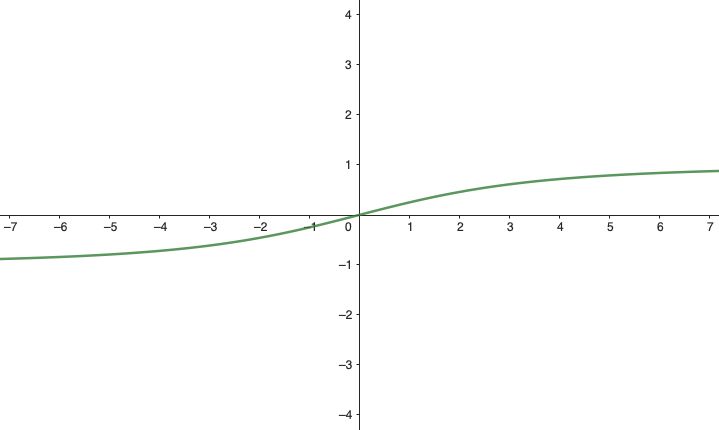
\includegraphics[width=0.98\textwidth]{gfx/grafica-normalizacion.png}
    \caption[Normalización utilizada con alfa como 15]{Normalización utilizada con alfa como 15.}\label{gfx:normalizacion}
\end{figure}

Se puede observar que a medida que \textit{x} crece, se acerca cada vez más a -1 o 1. Con un efecto similar, al usar muchas palabras en el sentimiento de \ac{VADER} se obtendrá una puntuación cercana a -1 o 1. Por lo tanto, el análisis de sentimientos de VADER funciona mejor en documentos cortos, como tweets o oraciones, no en documentos grandes.

\vspace{0.3cm}

Las características léxicas no es lo único que afecta al sentimiento de la oración. Existen otros elementos contextuales, como la puntuación, las mayúsculas y los modificadores que también imparten emoción. El análisis de sentimientos de \ac{VADER} los tiene en cuenta al considerar cinco heurísticas simples. El efecto de estas heurísticas se cuantifica, nuevamente, utilizando evaluadores humanos.

\vspace{0.3cm}

La primera heurística es la puntuación gramatical. Donde la oración \enquote{Me gusta}. expresa menos puntaje que \enquote{¡¡¡me gusta!!!}, esto es debido a que \ac{VADER} tiene en cuenta la cantidad de signos de exclamación y de interrogación que terminan la oración. \ac{VADER} primero calcula la puntuación de sentimiento de la oración. Si la puntuación es positiva, \ac{VADER} añade una cierta cantidad obtenida empíricamente por cada signo de exclamación (0,292) y signo de interrogación (0,18). Si la puntuación es negativa, entonces resta.

\vspace{0.3cm}

La segunda heurística es la capitalización. \enquote{INCREÍBLE actuación} es definitivamente más intenso que \enquote{increíble actuación}. Por ello, se aumenta o disminuye el puntaje de sentimiento de la palabra en 0.733, dependiendo de si la palabra es positiva o negativa, respectivamente. Esta característica no se ha implementado en mi proyecto, debido a que muchos tweets llevaban mayúsculas exclusivamente para llamar la atención y no para expresar sentimientos.

\vspace{0.3cm}

La tercera heurística es el uso de modificadores de grado. Por ejemplo, \enquote{muy lindo} y \enquote{más o menos lindo}. El efecto del modificador en la primera oración es aumentar la intensidad de lindo, mientras que en la segunda oración es disminuir la intensidad. \ac{VADER} mantiene un diccionario de refuerzo que contiene un conjunto de refuerzos y amortiguadores. Además, el efecto del modificador de grado también depende de su distancia a la palabra que está modificando. Las palabras más alejadas tienen un efecto intensificador relativamente menor sobre la palabra base. Un modificador al lado de la palabra suma o resta 0.293 al puntaje de sentimiento de la oración. Un segundo modificador de la palabra base suma o resta el 95\% de 0,293, y un tercero suma/resta el 90\%.

\vspace{0.3cm}

La cuarta heurística es el cambio de polaridad debido al \enquote{pero}. A menudo, \enquote{pero} conecta dos cláusulas con sentimientos contrastantes. El sentimiento dominante, sin embargo, es el último. Por ejemplo, \enquote{Te amo, pero ya no quiero estar contigo}. La primera frase \enquote{te amo} es positiva, pero la segunda \enquote{ya no quiero estar contigo}. es negativo y obviamente más dominante en cuanto al sentimiento. \ac{VADER} implementa un verificador de \enquote{pero}. Básicamente, todas las palabras sentimentales antes del \enquote{pero} tienen su valor reducido al 50\%, mientras que las que están después del \enquote{pero} aumentan al 150\%.

\vspace{0.3cm}

La quinta heurística es examinar el trigrama antes de una característica léxica cargada de sentimientos para captar la negación de la polaridad. Aquí, un trigrama se refiere a un conjunto de tres características léxicas. \ac{VADER} mantiene una lista de palabras negativas. La negación se captura multiplicando la puntuación de sentimiento de la característica léxica cargada de sentimiento por un valor determinado empíricamente -0,74.

\vspace{0.3cm}

Debido a todas estas características, la traducción del léxico inglés se ha realizado de una manera cuidadosa y selectiva (dejando las mismas puntuaciones que el léxico original), aunque se da por sentado que el léxico original tiene mayor capacidad de extraer los sentimientos. Sin embargo, la opción de traducir cada publicación iba a resultar mucho más costosa a la hora de ejecutarse. Primero la gran latencia de las múltiples traducciones que se puedan realizar y luego el limite de llamadas gratuitas diarias que claramente se van a traspasar.

\makeatletter
\let\orig@lstnumber=\thelstnumber

\newcommand\lstsetnumber[1]{\gdef\thelstnumber{#1}}
\newcommand\lstresetnumber{\global\let\thelstnumber=\orig@lstnumber}
\makeatother

\vspace{0.3cm}

\begin{lstlisting}[caption=Extracción de los sentimientos,          label={lst:listing-python},language=Python, mathescape=true]
def fetch_sentiments(query, lng, kw):

    if lng == 'es':
        analyzer = SentimentIntensityAnalyzerES()
    elif lng == 'uk':
        analyzer = SentimentIntensityAnalyzerUK()
    else:
        analyzer = SentimentIntensityAnalyzerEN()

    data: dict[str, list[list[float]]] = {
        'negative': [],
        'neutral': [],
        'positive': [],
    }

    try:
        if query:
            ppt = []
            for tweet in query:
                clean_txt = simple_clean(tweet.full_text)
                vader = round((analyzer.polarity_scores(clean_txt
                        ))['compound'], 4)
                y_axis = topic_relation(clean(clean_txt, lng),kw)
                popularity = ((tweet.retweet_count + 
                        tweet.favorite_count)*0.5)
                ppt.append(popularity)
                data = parse_data(data, vader, y_axis,popularity)$\lstsetnumber{\ldots}$
        $\lstresetnumber\setcounter{lstnumber}{45}$ 
        return data
    except Exception as e:

        print(e)
        return False
\end{lstlisting}

Como se ha explicado en la Historia de Usuario 11.1 (\ref{subs:sprint-8}) los sentimientos deberán estar representados en un gráfico. Por lo que los resultados proporcionados por \ac{VADER} pertenecerán al Eje X y la relación con las palabras clasificadas anteriormente será el Eje Y. Además, cada burbuja tiene un radio distinto, esto estará calculado conforme a la popularidad, es decir, si supera la popularidad media de la tendencia tendrá un radio más grande, pero también aumenta su radio si las coordenadas de las burbujas están muy cerca, para que no haya demasiadas repeticiones.

\vspace{0.3cm}

\begin{lstlisting}[caption=Extracción de las coordenadas de los sentimientos,          label={lst:extraccion-senti},language=Python, mathescape=true]
def parse_data(data, vader, y, ppt):
    if vader > 0.35:
        data['positive'].append([vader, y, ppt])
    elif vader < -0.35:
        data['negative'].append([vader, y, ppt])
    else:
        data['neutral'].append([vader, y, ppt])

    return data

def topic_relation(text, kw):
    suma = 0
    if len(text.split()):
        for k in kw:
            suma += text.split().count(k)
        relation = round(suma/len(text.split()), 4)
    else:
        relation = 0
    return relation

def fetch_sentiments(query, lng, kw):$\lstsetnumber{\ldots}$
    $\lstresetnumber\setcounter{lstnumber}{27}$
    m = np.max(ppt)
    a = round(np.average(ppt), 4)
    if m:
        for item in data.values():
            for k, i in enumerate(item):
                if i[2] > a:
                    i[2] = 2
                else:
                    i[2] = 1
                next = k + 1
    
                while next < len(item):
                    if round(i[0], 1) == round(item[next][0], 1)
                    and round(i[1], 1) == round(item[next][1],1):
                        i[2] = i[2] + 0.2
                        item.pop(next)
                    else:
                        next += 1
\end{lstlisting}

\subsection{Implementación de las Noticias}
La entidad de las noticias está compuesta por distintos valores comentados en la sección \ref{subsub:ent-noticias}. La estructuración de las noticias resulta tan sencilla como las que se han implementado anteriormente. Aunque la implementación tuvo varios cambios importantes.

\vspace{0.3cm}

\begin{lstlisting}[caption=Estructuración de las noticias,language=Python, mathescape=true]
# PARSING OBJECT WRAPPED
def parse_wrapped(item):

    date = item['date']
    image = item['image']
    summary = item['summary']
    title = item['title']
    url = item['url']
    source = item['source']

    values = {
        'date': date,
        'image': image,
        'summary': summary,
        'title': title,
        'url': url,
        'source': source
    }

    return Wrapped(**values)
\end{lstlisting}

Al empezar a implementar el código, pensé que la manera más sencilla de obtener información de noticias sería mediante una API. Aunque al usar distintas APIs sobre noticias, como \textit{News API} me di cuenta de que muchas noticias no estaban actualizadas, tenían errores en la descripción o el titulo y las APIs tenían por costumbre limitar drásticamente el número de peticiones por día.

\vspace{0.3cm}

Por ello tuve que cambiar el código y recurrir al scraping, una técnica utilizada para extraer información de sitios web. Para ello usé librerías como \textit{BeautifulSoup} o \textit{newspaper}, bibliotecas de Python para analizar documentos HTML y extraer de ellas información que resulte relevante.

\vspace{0.3cm}

Primero se descarga la búsqueda de noticias relevantes mediante el recurso XML de Google News. Esto se hace mediante los tópicos que se han extraído anteriormente y la biblioteca \textit{BeautifulSoup}, de esta manera las noticias serán mucho más refinadas. Además, siempre se intenta conseguir tres noticias diferentes y actuales, limitando la búsqueda por fecha.

\vspace{0.3cm}

Otro punto diferencial en la herramienta scraping y la API, es que con la herramienta scraping se conseguían artículos muchos más actuales y a la vez diferentes. Esto es debido a que al descargar artículos mediante la API solamente se podía condicionar el parámetro de búsqueda mediante la relevancia o actualidad, por lo que muchos artículos se podían repetir o quedaban desfasados. Gracias al scraping se pueden conseguir artículos recientes y a la vez relevantes, combinado los parámetros de búsqueda en Google News. Además, el problema de los artículos repetidos quedaba solucionado al usar un buscador más sotisficado que el de la API News.

\vspace{0.3cm}

\begin{lstlisting}[caption=Extracción de las noticias,language=Python, mathescape=true]
# GETTING ARTICLES
def get_everything(query, code, lang):
    # Getting the XML Content from Google News
    # An example: #https://news.google.com/rss/search?q=Riot+when:1d&hl=es&gl=ES&ceid=ES:es
    query = urllib.parse.quote(query.encode('utf8'))
    BASE_URL = f"https://news.google.com/rss/search?q={query}&hl={lang}&gl={code}&ceid={code}:{lang}"
    xml_content = requests.get(BASE_URL).content
    soup = BeautifulSoup(xml_content, features="xml")
    g_items = soup.find_all("item")

    if len(g_items) > 0:
        # Google Articles with poor info and not parsed yet
        g_articles = []
        for item in g_items:
            article = {}
            article["link"] = item.find("link").text
            article["title"] = item.find("title").text
            article["publisher"] = item.find("source").text
            article["published_date"] = item.find("pubDate").text
            g_articles.append(article)

        # Google with more info and parsed
        articles: list[dict[str, str]] = []
        cont = 0
        while len(articles) != 3 and cont < len(g_articles):
            article_info = get_article_info(g_articles[cont],
                        lang)
            if article_info:
                articles.append(article_info)
            cont += 1
        if len(articles) == 3:
            return articles
            
    return False
\end{lstlisting}

Al estar descargando información de Google News lo hacemos desde la ruta \textit{rss}. \ac{RSS} contiene un resumen de las actualizaciones de un sitio web y está escrito en XML. Una de las etapas más importantes del análisis de archivos XML es la búsqueda de etiquetas. Hay varias formas de hacer esto, mediante nombres o relaciones.

\vspace{0.3cm}

Al estar en recopilando información de una página simple y estática, como son los artículos de Google News se ha utilizado la extracción de información mediante nombres. La función de \textit{find} recibe el nombre de la etiqueta que desea obtener y devuelve un objeto BeautifulSoup de la etiqueta si encuentra uno, de lo contrario, devuelve \textit{None}.

\vspace{0.3cm}

De esta manera se puede realizar un bucle de todos los artículos relacionados con la tendencia. Consiguiendo información importante, como su enlace, el título, la editorial y la fecha de publicación.

\vspace{0.3cm}

Gracias a los artículos recopilados y sus enlaces correspondientes, podemos proseguir consiguiendo información relevante como una imagen de portada o la descripción.

\vspace{0.3cm}

\begin{lstlisting}[caption=Extracción de la información de las noticias,language=Python, mathescape=true]
# GETTING ARTICLES
def get_article_info(item, lang):
    user_agent = 'Mozilla/5.0 (Macintosh; Intel Mac OS X 10.15; rv:78.0) Gecko/20100101 Firefox/78.0'
    config = Config()
    config.browser_user_agent = user_agent
    config.request_timeout = 100
    config.MAX_TEXT = 500
    config.language = lang
    config.number_threads = 100
    a = Article(item["link"], language=lang, config=config)
    
    try:
        a.download()
        a.parse()
        date = parser.parse(item["published_date"])
        date_parsed = date.strftime("Date: %y-%m-%d Time: %H:%M")
        values = {
            'date': date_parsed,
            'image': a.top_image,
            'summary': a.text,
            'title': a.title,
            'url': item["link"],
            'source': item["publisher"]
        }
        if values["title"] and values["summary"] 
        and len(values["summary"].split()) > 20 
        and values["title"] != "Are you a robot?":
            return values
        else:
            return False
            
    except ArticleException as ae:
        print(ae)
        return False
        
    except Exception as e:
        print(e)
        return False
\end{lstlisting}

En esta sección de código, en vez de usar la biblioteca BeautifulSoup, se ha utilizado \textit{Newspaper3k}. Las ventajas de ello es que, la biblioteca Newspaper3k también puede realizar funciones más avanzadas, como descubrir fuentes RSS, buscar URL de artículos de una fuente de noticias principal e incluso extraer varios subprocesos si tiene que buscar más de un artículo. Además, termina siendo más conveniente al extraer información de sitios web diferentes.

\vspace{0.3cm}

Se ha establecido un gran tiempo para la conexión, para asegurar la descarga del articulo y su información, debido a esto el proceso de recopilación de datos sobre la tendencia resulta muy costoso. Aunque gracias al multiprocesamiento, se ha podido realizar las descargas de manera no secuencial y aligerar el proceso.

\vspace{0.3cm}

Después de añadir otras configuraciones como un \textit{header} para poder acceder a la página web sin limitaciones, se recopilan los diferentes datos y se estructuran de una manera conveniente. Además, pasan por validación por si la información recopilada no tiene sentido, en este caso la validación es bastante simple aunque efectiva. La descripción debe tener al menos 20 palabras, debe existir un título y que no sea \enquote{Are you a robot?}. La última validación es debido a que algunas páginas web comprueban cuidadosamente las peticiones que se hacen por estos métodos y devuelven esa información, en vez del articulo.

\subsection{Implementación del Servidor}
Anteriormente se ha descrito las diferentes implementaciones sobre las entidades, su estructuración y extracción de datos. Dichas implementaciones se encuentran en la carpeta \textit{app}, mientras que todo lo relacionado con el servicio del servidor se encuentra en el directorio \textit{backend}. No entraré en mucho detalle en la implementación de las clases o rutas, ya que se han explicado en la sección de diseño (\ref{ch:diseño}). Aunque interferiré en el modelo \textit{Country} y su obtención.

\vspace{0.3cm}

\begin{lstlisting}[caption=Modelo \textit{Country} y ejemplo de ruta,language=Python, mathescape=true]
class Country(BaseModel):
    id: str = Field(default_factory=uuid.uuid4, alias="_id")
    pais: str = Field(...)
    dia: str = Field(...)
    tendencias: List[Trend] = Field(...)

    class Config:
        allow_population_by_field_name = True
        schema_extra = {
            "example": {
                "_id": "066de609-b04a-4b30-b46c-32537c7f1f6e",
                "pais": "Spain",
    $\lstsetnumber{\ldots}$
    $\lstresetnumber\setcounter{lstnumber}{0}$

@router.get("/{name}/{date}", response_description=
    "Get a single country by the name and date",
    response_model=Country)
def find_country(name: str, date: str, request: Request):
    if (country := request.app.database["countries"].find_one(
    {"pais": name, "dia": date})) is not None:
        country["tendencias"] = list(
            filter(itemgetter("wrappeds"),
            country["tendencias"]))[:10]
        return country

    raise HTTPException(status_code=status.HTTP_404_NOT_FOUND,
                        detail=f"Country with the name {name} 
                        and date {date} not found")
\end{lstlisting}

La ruta devuelve un objeto bajo el modelo de \textit{Country} mediante la fecha y el nombre del país, tal y como se ha explicado en la sección de diseño de interacción de rutas (diagrama \ref{gfx:diagrama-itr4}). Todas las demás rutas y entidades tienen un comportamiento parecido. La peculiaridad de esta ruta es que filtra diez tendencias que tengan el objeto de noticias o \textit{wrappeds}, para no mostrar tendencias vacías.

\section{Implementación Front-end}
La implementación de la capa de \textit{Front-end} se localiza bajo el directorio \textit{front-end}, la estructura de la aplicación de Vue sigue las buenas prácticas conteniendo archivos correspondientes en cada directorio relevante a la aplicación, es decir, se han separado en \textit{assets}, \textit{components}, \textit{router}, \textit{styles} y la carpeta \textit{public}.

\subsection{Implementación Principal}
La primera implementación de código que se estudiará será la vista principal descrita anteriormente en la sección \ref{subs:vista-principal}. Cabe mencionar que no se podrá estudiar todo el código, debido a que incluir todas las reglas de diseño CSS y la estructura HTML complicarían la lectura y su propia comprensión. Aunque indagaré en las diferencias más destacables.

\vspace{0.3cm}

La estructura de un archivo Vue se compone de tres apartados esenciales, el primer apartado llamado \textit{template} contiene la implementación HTML, el segundo llamado \textit{script} contendrá implementaciones de JavaScript y por último \textit{style} incluirá implementaciones de diseño.

\vspace{0.3cm}

\begin{lstlisting}[caption=Secciones de Vue,language=Python, mathescape=true]
<template>$\lstsetnumber{\ldots}$
        $\lstresetnumber\setcounter{lstnumber}{120}$
          <div class="flex overflow-x-auto gap-6 snap-x snap-mandatory sm:snap-normal before:shrink-0 before:w-[20%] sm:before:w-[0%] after:shrink-0 after:w-[20%] sm:after:w-[0%] sm:horizontal sm:pb-14 pb-5">
            <div
              v-if="articulos.popularity"
              class="basis-4/5 sm:basis-3/12 xl:basis-2/12 shrink-0 snap-center sm:snap-align-none shadowdrop"
            >
              <GraphViewer
                :array-popularity="articulos.popularity.volume"
                :array-hours="articulos.popularity.hour_popularity"
                :avarage-popularity="articulos.popularity.avarage_popularity"
                :peak-popularity="articulos.popularity.peak_popularity"
                :num="1"
                :rank="index+1"
                :url="encondeURL(articulos.name)"
              />
            </div>$\lstsetnumber{\ldots}$
                    $\lstresetnumber\setcounter{lstnumber}{163}$
</template>

<script>
import axios from 'axios';$\lstsetnumber{\ldots}$
$\lstresetnumber\setcounter{lstnumber}{270}$
export default {
  components: {
    CardViewer,
    GraphViewer,
    MapViewer,
    BubbleViewer,
  },$\lstsetnumber{\ldots}$
$\lstresetnumber\setcounter{lstnumber}{410}$
</script>

<style>$\lstsetnumber{\ldots}$
$\lstresetnumber\setcounter{lstnumber}{425}$
.truncador-title {
  overflow: hidden;
  display: -webkit-box;
  -webkit-box-orient: vertical;
  -webkit-line-clamp: 2;
  -webkit-margin-collapse: discard;
}$\lstsetnumber{\ldots}$
$\lstresetnumber\setcounter{lstnumber}{570}$
</style>

\end{lstlisting}

En la sección \textit{template} de esta vista se encuentra toda la estructura HTML de la página y llamadas a otros componentes. Gracias a funciones Vue se ha podido implementar bucles o funciones directamente en dicha estructura. Un ejemplo de ello es el \textit{v-if} o \textit{v-for} los cuales renderizan contenido mediante condiciones o listas. La renderización de listas fue algo esencial a la hora de renderizar un \ac{JSON} devuelto de la base de datos.

\vspace{0.3cm}

Luego, en la sección de \textit{script} se implementa la parte programable. En el caso de la vista principal se realizan llamadas a la base de datos justo en la creación de la página web, esto es debido a que el contenido se cargue justo al inicio de la creación de la página web, sin tener que esperar a la carga de todos los componentes necesarios como se puede ver en el esquema posterior.

\begin{figure}[H]
    \centering
    \myfloatalign
    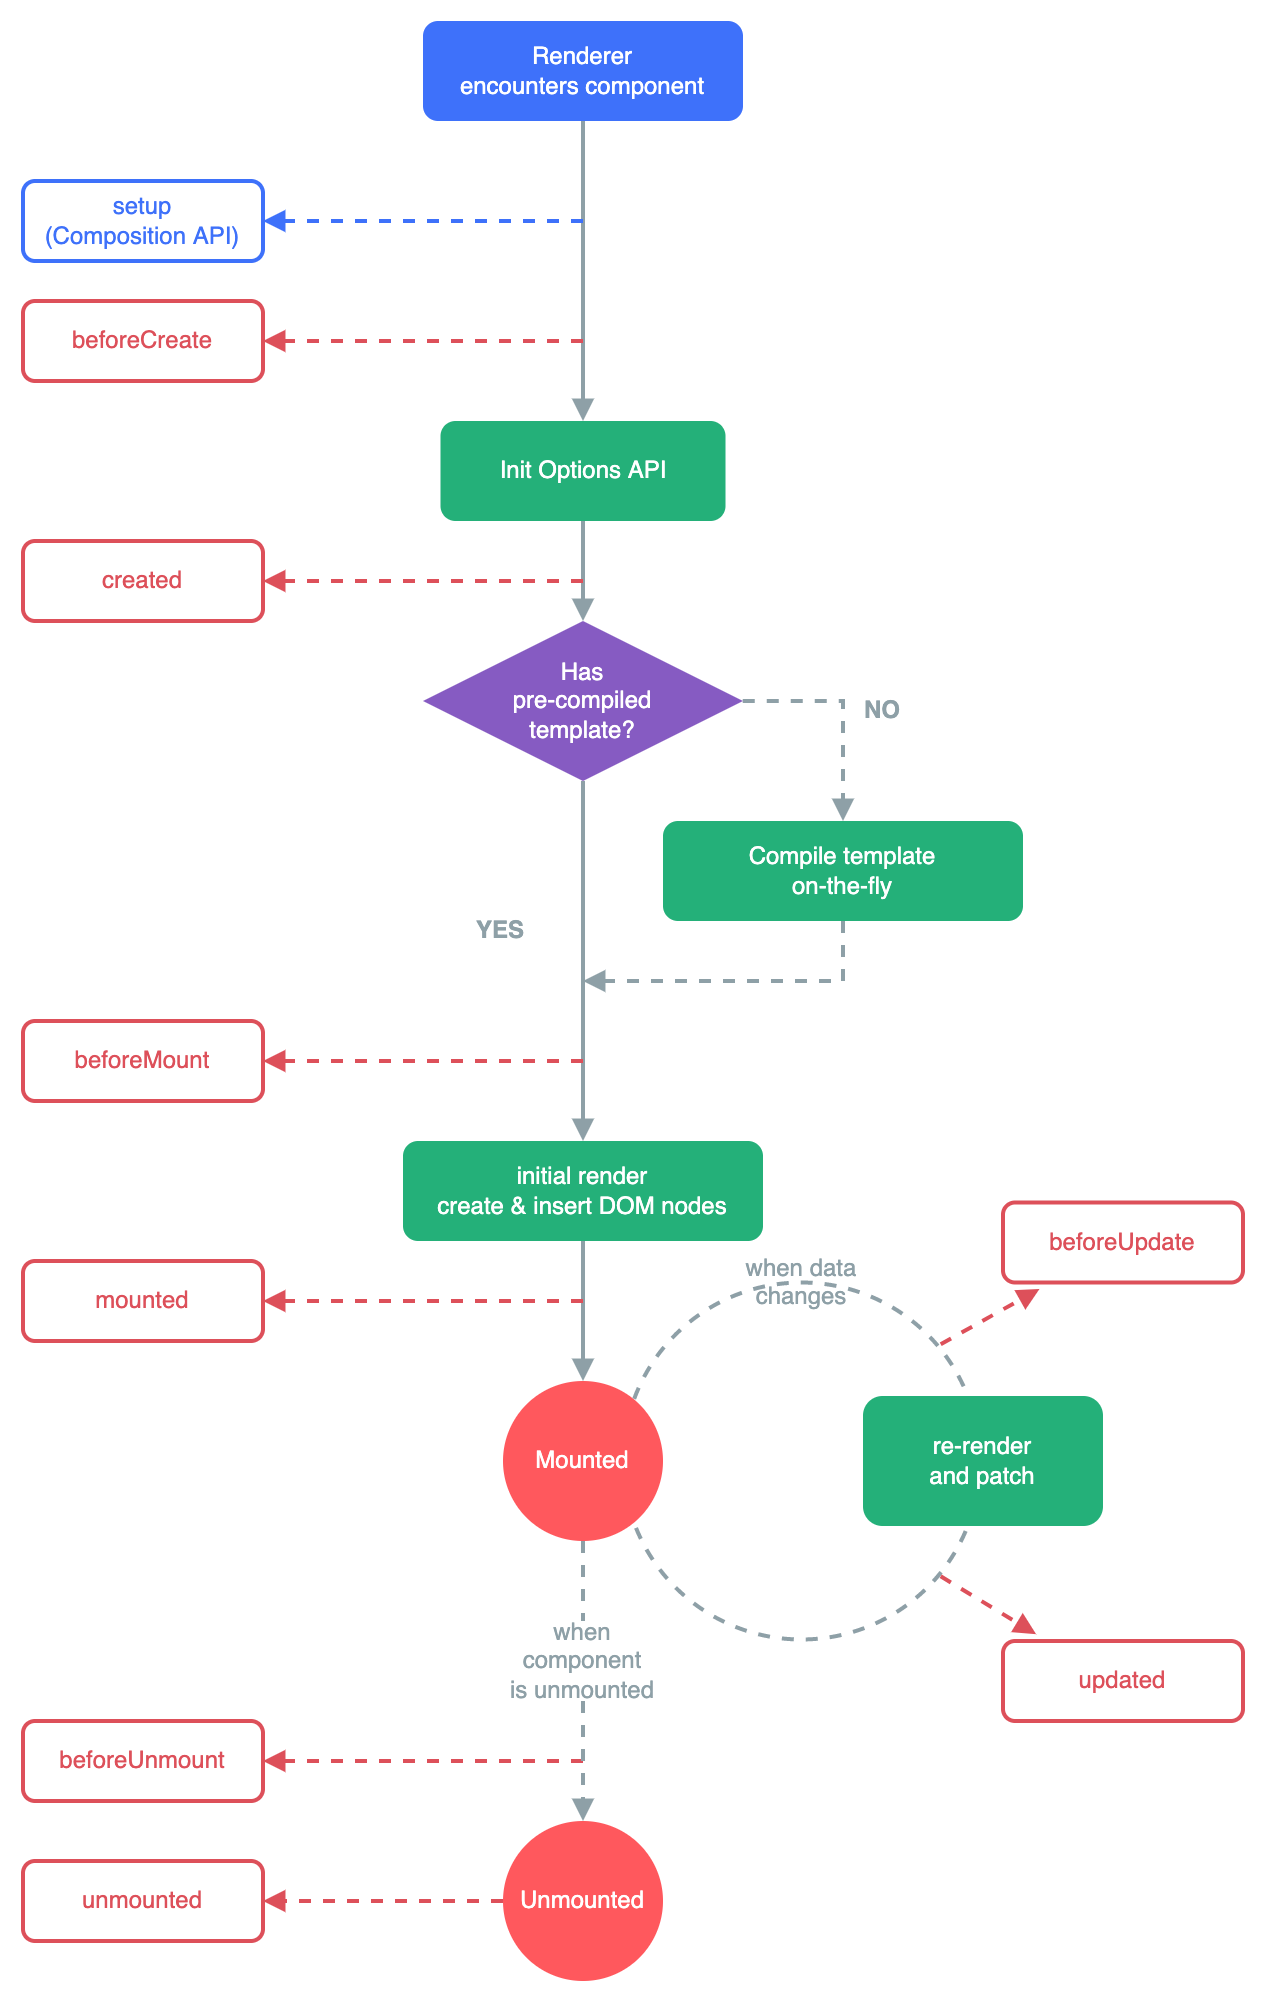
\includegraphics[width=0.82\textwidth]{gfx/lifecyclevue.png}
    \caption[Ciclo de vida de una aplicación Vue]{Ciclo de vida de una aplicación Vue \cite{vue-life}.}\label{gfx:lifecyclevue}
\end{figure}

El código mostrado es una versión simplificada, con el objetivo de facilitar la comprensión. Lo importante del código es que se ha implementado un manejo de errores y la creación de contenido de la página dependiendo de la URL que se haya introducido.

\vspace{0.3cm}

\begin{lstlisting}[caption=Funciones de carga de contenido en Vue,language=Python, mathescape=true]
async created() {
    await this.fetch();
},
methods: {
    async fetch() {
      this.loading = true;
      try {
        let data = {};
        if (this.route.query.name and this.route.query.query) {
          data = await axios.get((`{SEARCHTRENDINGENDPOINT}`));
        } else { data = await axios.get((`{TRENDINGENDPOINT`));}
        if (data.status === 200 and data.data.
            tendencias[0].wrappeds) {
          this.wrapped = data.data.tendencias;
          this.loading = false;
          this.error = false;
        } else {
          this.country = 'Spain';
          this.date = this.dateString(new Date());
          this.alert('There was an error trying to load (...)');
        }
      } catch (error) {
        this.country = 'Spain';
        this.date = this.dateString(new Date());
        this.alert('Right now it looks like the web is (...)');
        console.log(error);
      }
    },
},
\end{lstlisting}

Otra sección a destacar el el diseño. La implementación de esta sección tuvo el mismo o incluso más arduo trabajo que las demás, primero al querer tener un diseño original y que funcionase en todos los dispositivos, se han implementado muchísimas reglas en CSS, entre ellas reglas de medida o consultas de medio para cambiar toda la visualización de contenido dependiendo de la medida del dispositivo. 

\vspace{0.3cm}

Esto es debido a que se ha querido que se viera de una manera óptima sin sacrificar la visibilidad del contenido. Por ello se ha recurrido a herramientas como el truncamiento en CSS. Luego otro de los detalles del diseño es que las sombras varían dependiendo del navegador, debido al rendimiento que tienen sobre estos. El navegador Chrome llega a funcionar muy bien con la opción \textit{filter()} de CSS, pero sin embargo Safari no. También hay que tener en cuenta las personas que tengan el zoom activado en el teléfono y adaptar también su contenido, incluso pantallas gigantes o extremadamente pequeñas, todo esto hace que el diseño pueda ser debidamente \textit{responsive}.

\vspace{0.3cm}

Otro detalle, a parte de las sombras, es que, en los dispositivos no móviles, se han implementado animaciones de \textit{hover}. Estas animaciones levantan y oscurecen ligeramente la carta o módulo cada vez que el ratón pasa por encima, facilitando así su visualización.

\vspace{0.3cm}

También se han seguido las buenas prácticas y se ha respetado el contraste de los colores para la una lectura más fácil de los enlaces web o el propio contenido de la página. Además, se han usado varios \textit{svg} con formas de ola, para que la página sea más agradable a la vista.

\vspace{0.3cm}

\begin{lstlisting}[caption=Detalles de la implementación del diseño,language=Python, mathescape=true]
@media (min-height: 550px) {
  contenido {
    height: 10rem;
  }

  .truncador {
    overflow: hidden;
    display: -webkit-box;
    -webkit-box-orient: vertical;
    -webkit-line-clamp: 5;
    -webkit-margin-collapse: discard;
  }$\lstsetnumber{\ldots}$
$\lstresetnumber\setcounter{lstnumber}{37}$
}

/* Safari 10.1+ */
@media not all and (min-resolution:.001dpcm) { @media {
  .shadowdrop {
    filter: none;
    -webkit-filter: none;
    -moz-filter:  none;
    -ms-filter:  none;
    -o-filter: none;
    box-shadow: rgba(0, 0, 0, 0.03) 0px 15px 7px -7px;
  }
}}
\end{lstlisting}

\subsection{Implementación de la Popularidad}
El código implementado en esta sección se refiere a la subvista popularidad explicada en la sección \ref{subs:vista-popu}. Las principales diferencias de implementación en este módulo es la implementación de diferentes funciones en el \textit{template} de la vista y también la propia implementación del gráfico, ya que es una librería que requiere mucha personalización para poderse visualizar adecuadamente.

\vspace{0.3cm}

\begin{lstlisting}[caption=Diferencias destacables de la implementación de la popularidad,language=Python, mathescape=true]
<ul class="text-sm contenido-stats text-ellipsis overflow-hidden">
  <li class="py-0.5 pt-1">
    - First data at {{ encondeHour(arrayHours[0]) }}.
  </li>
  <li class="py-0.5">
    - Last data at
    {{ encondeHour(arrayHours[arrayHours.length - 1]) }}.
  </li>
  <li class="py-0.5">
    - Peak popularity is {{ peakPopularity.toLocaleString('en-US') }}.
  </li>
  <li class="py-0.5 pb-1">
    - Average popularity is {{ avaragePopularity.toLocaleString('en-US') }}.
  </li>
</ul>$\lstsetnumber{\ldots}$
$\lstresetnumber\setcounter{lstnumber}{62}$
chartOptions: {
    chart: {
      type: 'area',
      toolbar: {
        show: false,
      },
      zoom: {
        enabled: false,
      },
      animations: { enabled: false },
    },
    xaxis: {
      type: 'datetime',
      categories: this.arrayHours,
      labels: {
        format: 'HH:mm',
        },$\lstsetnumber{\ldots}$
        $\lstresetnumber\setcounter{lstnumber}{94}$
        markers: {
          size: 3,
        },
      },
\end{lstlisting}

Las horas en este caso se guardan en formato JavaScript y se transforman en objeto \textit{date} al implementarlo en el código Vue. Además, se ha respetado las horas locales de cada país como se puede ver en el código.

\vspace{0.3cm}

En el siguiente ejemplo de visualización, se ha usado el navegador de Chrome bajo la premisa de simular la vista de un iPhone SE (un teléfono bastante compacto). El contenido que se puede visualizar es el descenso de popularidad que tuvo la tendencia \textit{Joji}. Podemos ver cómo empezó siendo popular sobre la madrugada, pero que poco a poco fue decayendo. En el día de 5 de noviembre, se encuentra en la octava posición del top 10 tendencias más populares de España. El valor del volumen de publicaciones, es decir el número de veces que se ha mencionado la tendencia fue de 86,748 como máximo y 59,957 de media.

\begin{figure}[H]
    \centering
    \myfloatalign
    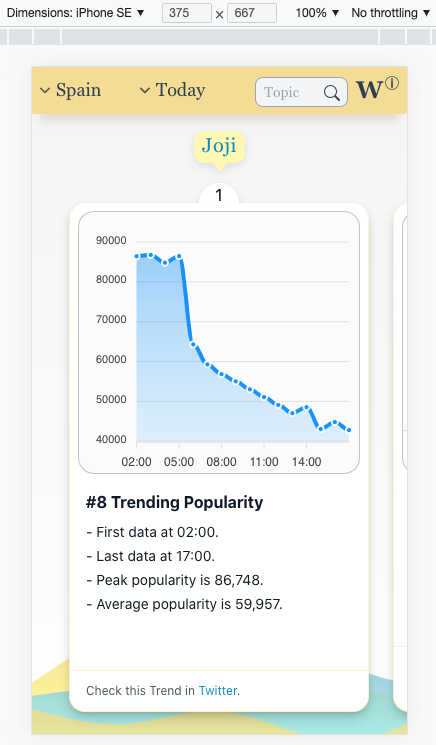
\includegraphics[width=0.75\textwidth]{gfx/ejemplo2.png}
    \caption[Ejemplo de tendencia, vista de popularidad]{Ejemplo de tendencia, vista de popularidad.}\label{gfx:ejemplo2}
\end{figure}

\subsection{Implementación de las \textit{Keywords}}
El código implementado en esta sección se refiere a la subvista \textit{keywords} explicada en la sección \ref{subs:vista-key}. En cuanto a las principales diferencias, es la cantidad de código que ha requerido la implementación de la personalización del gráfico.

\vspace{0.3cm}

\begin{lstlisting}[caption=Diferencias destacables de la implementación de las keywords,language=Python, mathescape=true]
series: this.arrayCount,
chartOptions: {
chart: {
  type: 'radialBar',
  toolbar: {
    show: false,
  },
  animations: { enabled: false },
  sparkline: {
    enabled: true,
  },
},
colors: [
  '#008FFB',
  '#00E396',
  '#FEB019',
  '#FF4560',
  '#775DD0',
  '#5DABD0',
],
plotOptions: {
  radialBar: {
    offsetY: -5,
    startAngle: 0,
    endAngle: 360,
    hollow: {
      margin: 5,
      size: '0%',
      background: 'transparent',
    },
$\lstsetnumber{\ldots}$
$\lstresetnumber\setcounter{lstnumber}{0}$
\end{lstlisting}

Los colores y sombras han sido definidos manualmente, al igual que la posición del gráfico y el etiquetado de sus datos.

\vspace{0.3cm}

En el siguiente ejemplo podemos visualizar el contexto de la tendencia. Obviamente el nombre de la tendencia es la palabra que más se repite en las publicaciones, se ha repetido 99 veces en los 100 tweets recopilados. Para entender la situación podemos ver las palabras más repetidas y los \textit{keywords}, la información que nos dan es «Album De Joji», «Die For You» y «Nuevo Disco». Al parecer Joji es un cantante o al menos una persona famosa, que ha sacado un disco o álbum nuevo llamado "Die For You".

\begin{figure}[H]
    \centering
    \myfloatalign
    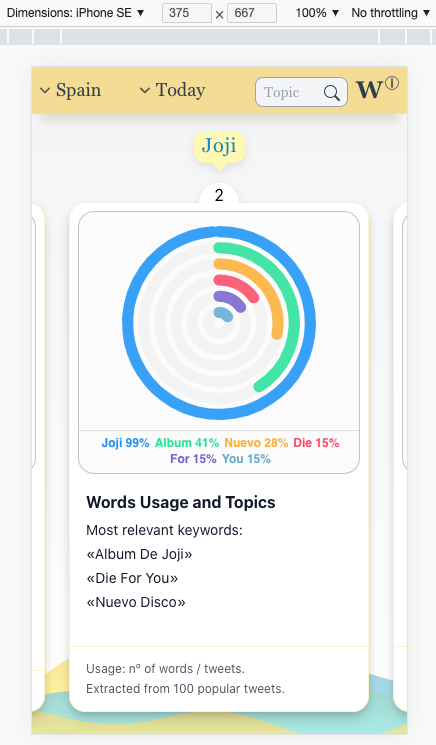
\includegraphics[width=0.75\textwidth]{gfx/ejemplo3.png}
    \caption[Ejemplo de tendencia, vista de \textit{keywords}]{Ejemplo de tendencia, vista de \textit{keywords}.}\label{gfx:ejemplo3}
\end{figure}

\subsection{Implementación de los Sentimientos}
El código implementado en esta sección se refiere a la subvista sentimientos explicada en la sección \ref{subs:vista-senti}. Aquí también destaca la implementación la personalización del gráfico, aunque también hay funciones que requieren explicación.

\vspace{0.3cm}

Todos los ejes, el marco o las propias burbujas han tenido su implementación de posición, color y grosor de trazado. Además, el lienzo en el que se pinta es algo más grande que la notación del etiquetado, esto es debido a que se pretende que se visualice mejor la gráfica y no se corten las burbujas.

\vspace{0.3cm}

\begin{lstlisting}[caption=Diferencias destacables de la implementación de los sentimientos,language=Python, mathescape=true]
xaxis: {
  min: -1,
  max: 1,
  tickAmount: 1,
  type: 'numeric',
  position: 'bottom',
  decimalsInFloat: 0,
  labels: {
    offsetY: -4,
    style: {
      fontSize: '11px',
    },
  },
  axisBorder: {
    show: false,
  },
  axisTicks: {
    show: false,
  },
  title: {
    text: 'Compound',
    offsetY: -22,
    style: {
      fontSize: '12px',
      fontWeight: 350,
    },
  },
},
$\lstsetnumber{\ldots}$
$\lstresetnumber\setcounter{lstnumber}{132}$
percentageSentiment(array, arrayA, arrayB) {
  let suma = 0;
  let val = 0;
  array.forEach((item) => {
    suma += item[2];
  });
  val = suma;
  arrayA.forEach((item) => {
    suma += item[2];
  });
  arrayB.forEach((item) => {
    suma += item[2];
  });
  return (Math.round((val / suma) * 100));
},
\end{lstlisting}

El porcentaje se calcula en torno al radio de la burbuja, ya que no tiene sentido calcular la cantidad de burbujas porque como se ha explicado en la sección de su implementación (\ref{lst:extraccion-senti}) se eliminan las que tienen coordenadas muy similares.

\vspace{0.3cm}

En el ejemplo siguiente, del cantante Joji, la mayoría de las publicaciones tienen que ser positivas debido a los seguidores de esta persona, al comprobarlo vemos que efectivamente el 56\% son publicaciones positivas. También puede haber publicaciones negativas o neutras, tal como análisis de críticos que no expresan una opinión o personas a las que no les ha gustado. Claramente también puede haber errores, ya que la extracción del sentimiento no es cien por cien precisa, aunque se puede ver que el sentimiento global es acertado.

\begin{figure}[H]
    \centering
    \myfloatalign
    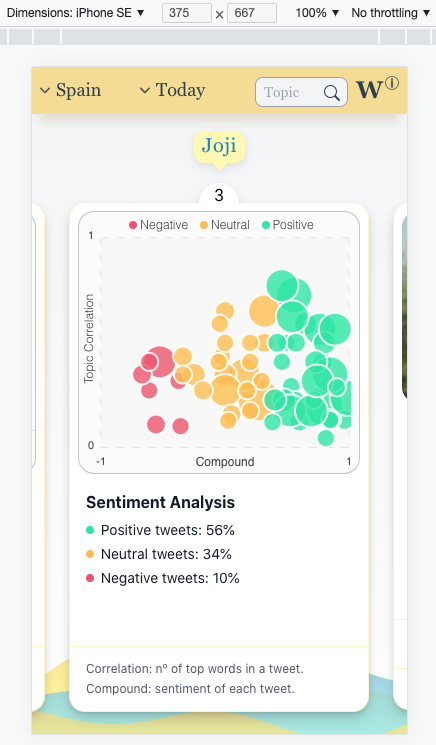
\includegraphics[width=0.75\textwidth]{gfx/ejemplo4.png}
    \caption[Ejemplo de tendencia, vista de sentimientos]{Ejemplo de tendencia, vista de sentimientos.}\label{gfx:ejemplo4}
\end{figure}

También se puede comprobar por tweets o publicaciones específicas, ya que cada burbuja es una:

\vspace{0.3cm}

\begin{quotation}
		\textit{"lo siento jefe hoy no puedo trabajar el album de joji me ha puesto triste"}
\end{quotation}
Puntuación: -0.7061

\vspace{0.4cm}

Podemos ver y comprobar la publicación en la propia plataforma.

\begin{figure}[H]
    \centering
    \myfloatalign
    
\includegraphics[width=0.95\textwidth]{gfx/twit1.png}
    \caption[Ejemplo de tweet (1)]{Ejemplo de tweet (1).}\label{gfx:twit1}
\end{figure}

\vspace{0.3cm}

\begin{quotation}
		\textit{"hoy es un buen dia porque joji saco un nuevo album con musica muy buena, asi que, buenos dias; escuchen a joji, es arte."}
\end{quotation}
Puntuación: 0.902

\vspace{0.4cm}

El sentimiento en este caso también es justificado. Podemos ver y comprobar la publicación en la propia plataforma.

\begin{figure}[H]
    \centering
    \myfloatalign
    
\includegraphics[width=0.95\textwidth]{gfx/twit2.png}
    \caption[Ejemplo de tweet (2)]{Ejemplo de tweet (2).}\label{gfx:twit2}
\end{figure}

\vspace{0.3cm}

\begin{quotation}
		\textit{"toca llorar toda la noche escuchando el nuevo album de joji en loop"}
\end{quotation}
Puntuación: -0.34

\vspace{0.3cm}

El sentimiento en este caso también es justificado, aunque obviamente es una publicación sarcástica, algo que la herramienta de extracción no entendería.

\vspace{0.3cm}

Lo bueno de comprobar estas publicaciones que las imágenes u otros elementos como los \textit{hashtags} no interfieren en el análisis de sentimientos. Además, se recogen publicaciones con mucha interacción, tal y como lo hemos especificado en el algoritmo.

\vspace{0.1cm}

\begin{figure}[H]
    \centering
    \myfloatalign
    
\includegraphics[width=0.81\textwidth]{gfx/twit3.png}
    \caption[Ejemplo de tweet (3)]{Ejemplo de tweet (3).}\label{gfx:twit3}
\end{figure}

\subsection{Implementación de las Noticias}
El código implementado en esta sección se refiere a la subvista \textit{keywords} explicada en la sección \ref{subs:vista-noti}. En cuanto a las principales diferencias, no destaca mucho en la implementación, ya que solo tiene que mostrar valores proporcionados de la página web, pero destaca en el diseño.

\vspace{0.3cm}

Las animaciones y otros detalles parten de esta vista. También existe una función que, ante un fallo de carga de imagen, provee una imagen por defecto para las noticias.


\vspace{0.3cm}

\begin{lstlisting}[caption=Diferencias destacables de la implementación de las noticas,language=Python, mathescape=true]
import img from '../assets/img_news.jpg';
export default {
  methods: {
    replaceByDefault(e) {
      e.target.src = img;
    },
  },
$\lstsetnumber{\ldots}$
$\lstresetnumber\setcounter{lstnumber}{122}$
@media (hover: hover) and (pointer: fine) {
  .animation:hover {
    --tw-translate-y: -0.5rem /* -8px */;
    transform: translate(var(--tw-translate-x), var(--tw-translate-y))
      rotate(var(--tw-rotate)) skewX(var(--tw-skew-x)) skewY(var(--tw-skew-y))
      scaleX(var(--tw-scale-x)) scaleY(var(--tw-scale-y));
  }
  .animation-shadow:hover {
    --tw-shadow: 0 20px 25px -12px rgb(0 0 0 / 0.35);
    --tw-shadow-colored: 0 20px 25px -12px var(--tw-shadow-color);
    box-shadow: var(--tw-ring-offset-shadow, 0 0 #0000),
      var(--tw-ring-shadow, 0 0 #0000), var(--tw-shadow);
  }
}
\end{lstlisting}

Hay tres noticias bastante parecidas. Las tres anuncian el nuevo álbum, a lo mejor también información sobre sus conciertos o donde poder escucharlo.

\begin{figure}[H]
    \centering
    \myfloatalign
    
\includegraphics[width=0.75\textwidth]{gfx/ejemplo5.png}
    \caption[Ejemplo de tendencia, vista de noticias]{Ejemplo de tendencia, vista de noticias.}\label{gfx:ejemplo5}
\end{figure}

La noticia presenta un titulo, descripción y fotografía explicativa. La fotografía es del cantante Joji. Se puede acceder a dicho articulo mediante el enlace de la editorial o directamente pulsando sobre la foto.

\begin{figure}[H]
    \centering
    \myfloatalign
    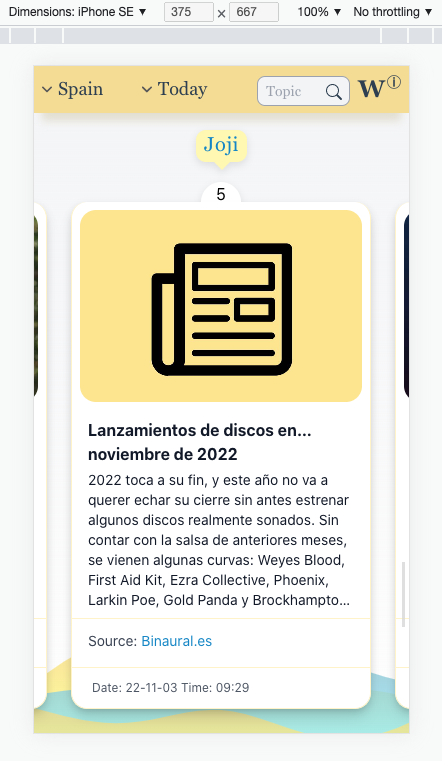
\includegraphics[width=0.75\textwidth]{gfx/ejemplo6.png}
    \caption[Ejemplo de tendencia, vista de noticias por defecto]{Ejemplo de tendencia, vista de noticias por defecto.}\label{gfx:ejemplo6}
\end{figure}

La búsqueda por tópicos funcionaria de la misma manera. Como ultima mención, la implementación de errores fue implementada tal cual descrita en la sección \ref{gfx:boceto-error}. El mensaje de la alerta cambia dependiendo del error ocurrido, para que el usuario tenga conciencia de cuál fue el problema. 